\begin{figure}[tp]
    \begin{minipage}[h]{0.5\linewidth}
    \center{
        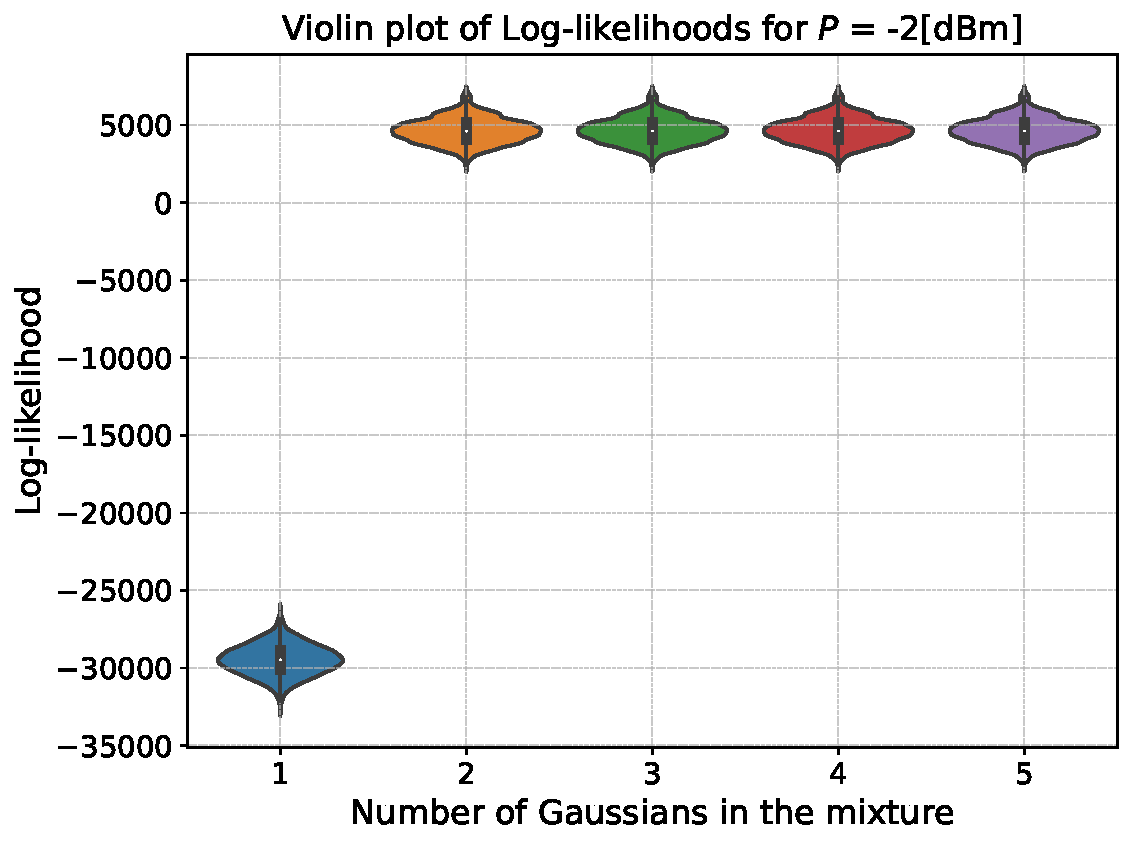
\includegraphics[width=1\linewidth]{images/gauss/bigf_loglik_pdbm_-2.pdf} (a) \\
    }
    \end{minipage}
    \begin{minipage}[h]{0.5\linewidth}
    \center{
        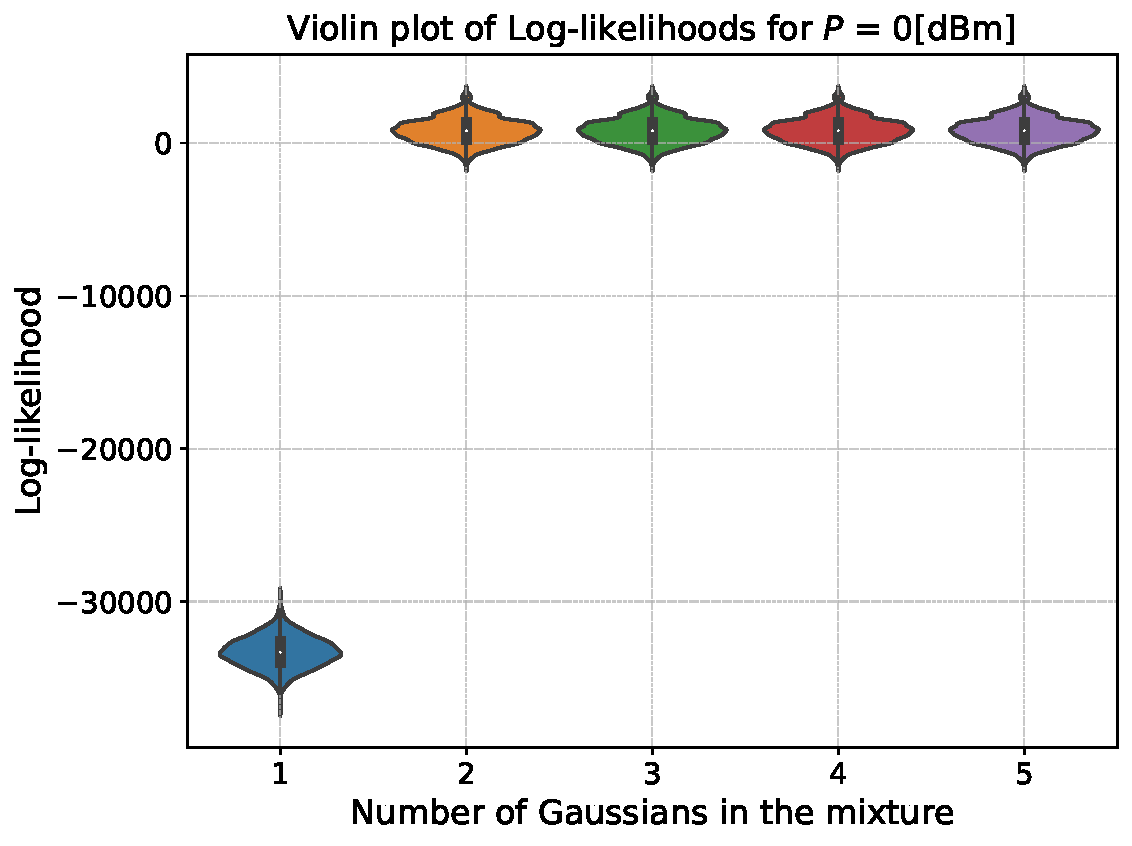
\includegraphics[width=1\linewidth]{images/gauss/bigf_loglik_pdbm_0.pdf} (b) \\
    }
    \end{minipage}

    \begin{minipage}[h]{0.5\linewidth}
    \center{
        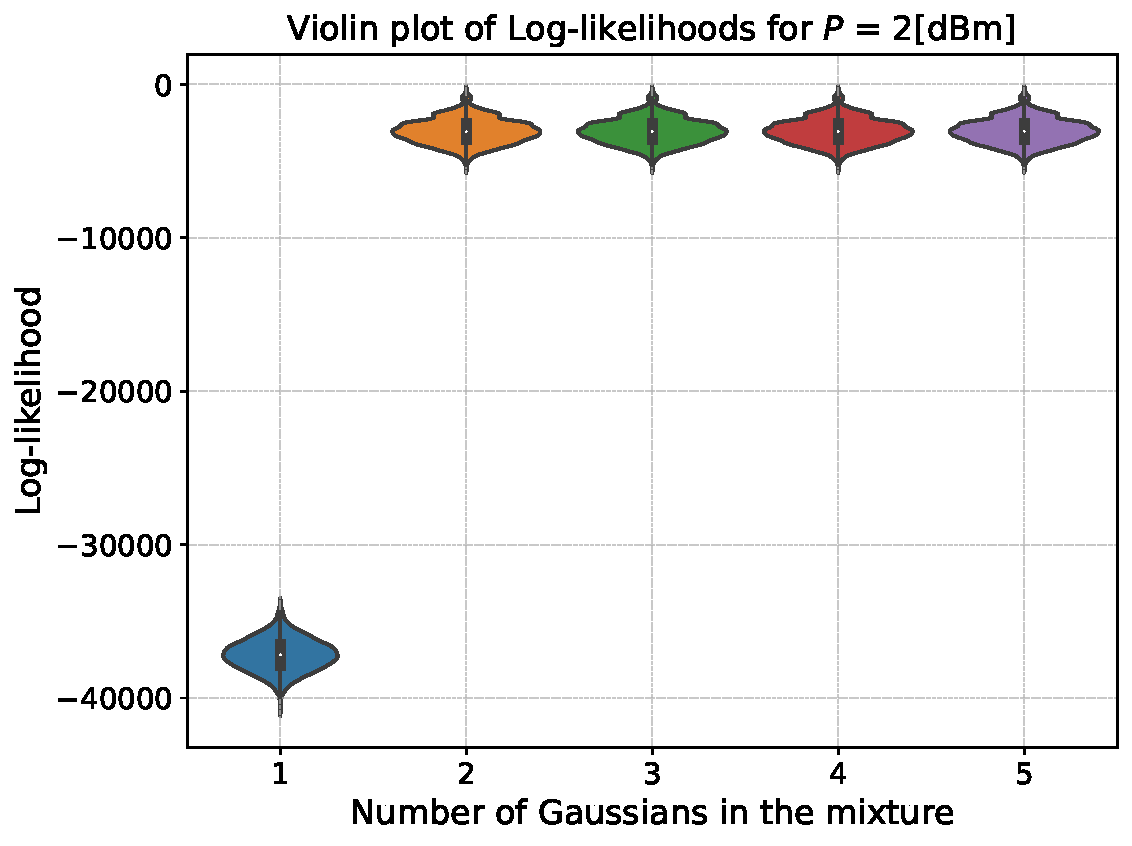
\includegraphics[width=1\linewidth]{images/gauss/bigf_loglik_pdbm_2.pdf} (c) \\
    }
    \end{minipage}
    \begin{minipage}[h]{0.5\linewidth}
    \center{
        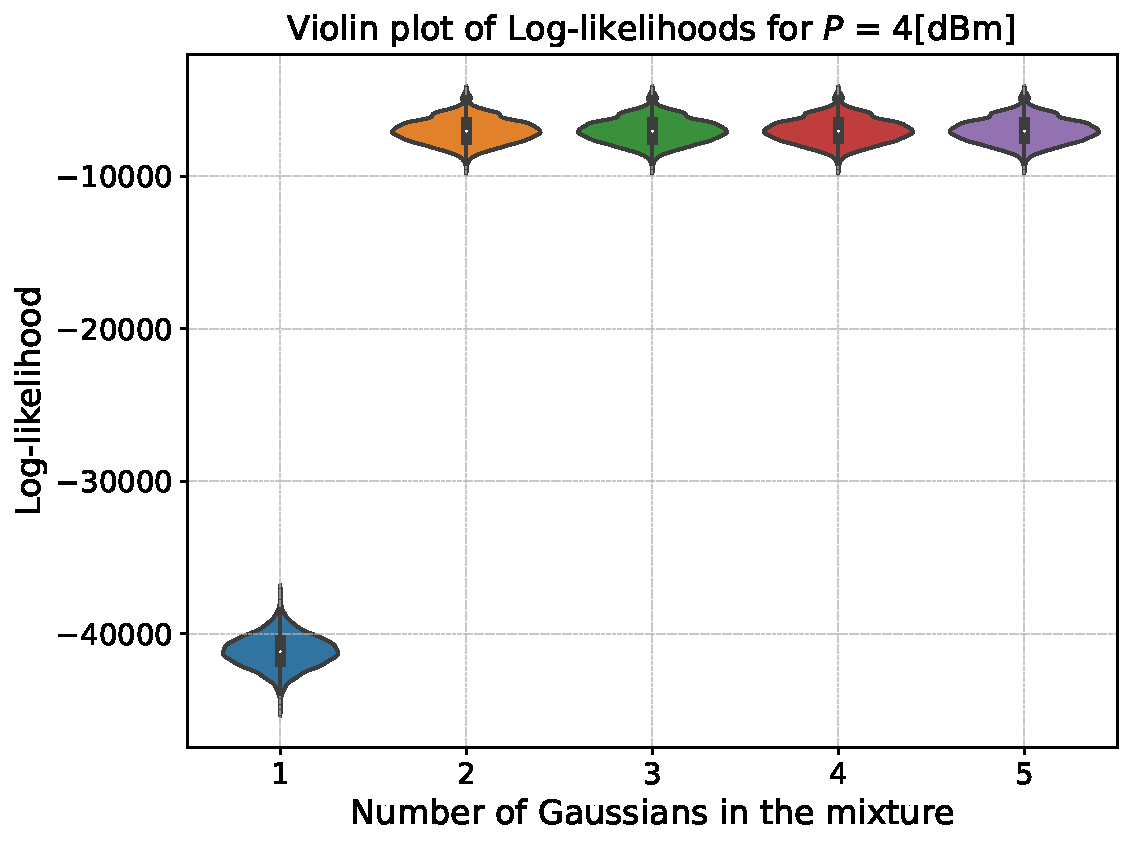
\includegraphics[width=1\linewidth]{images/gauss/bigf_loglik_pdbm_4.pdf} (d) \\
    }
    \end{minipage}

    \begin{minipage}[h]{0.5\linewidth}
    \center{
        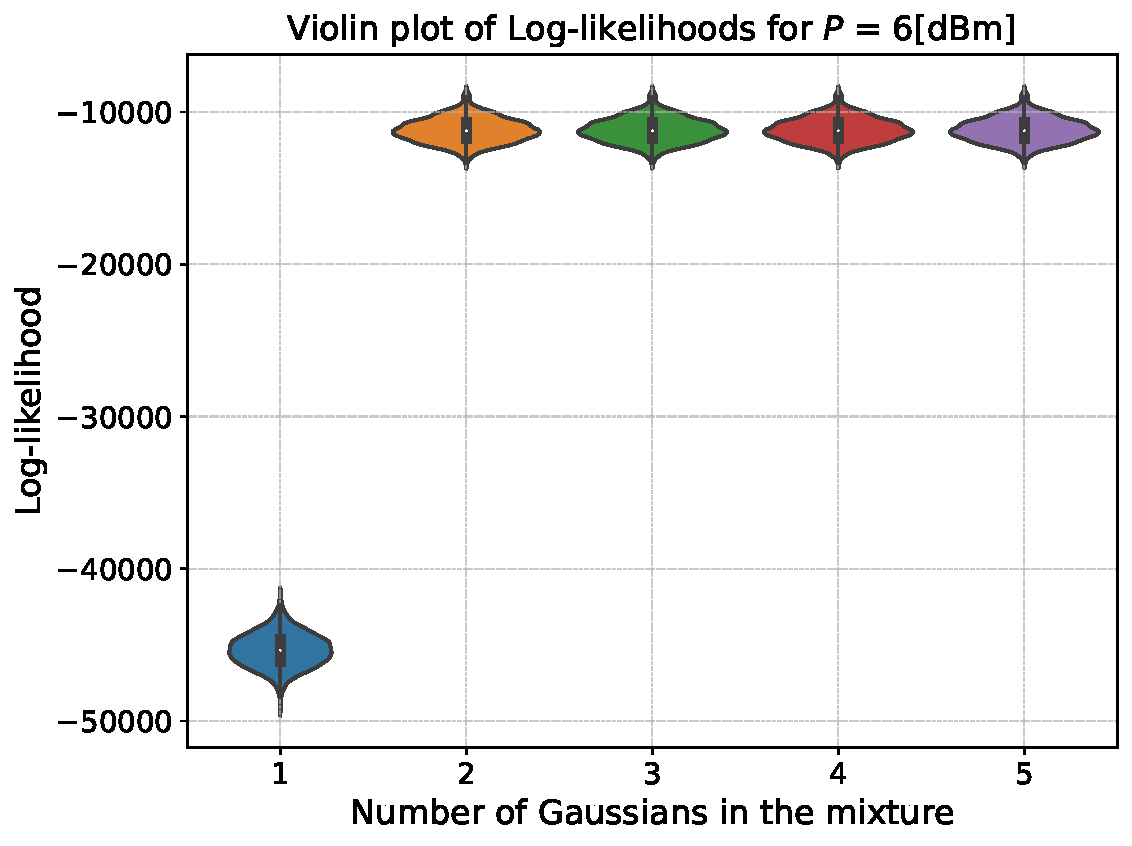
\includegraphics[width=1\linewidth]{images/gauss/bigf_loglik_pdbm_6.pdf} (e) \\
    }
    \end{minipage}
    \begin{minipage}[h]{0.5\linewidth}
    \center{
        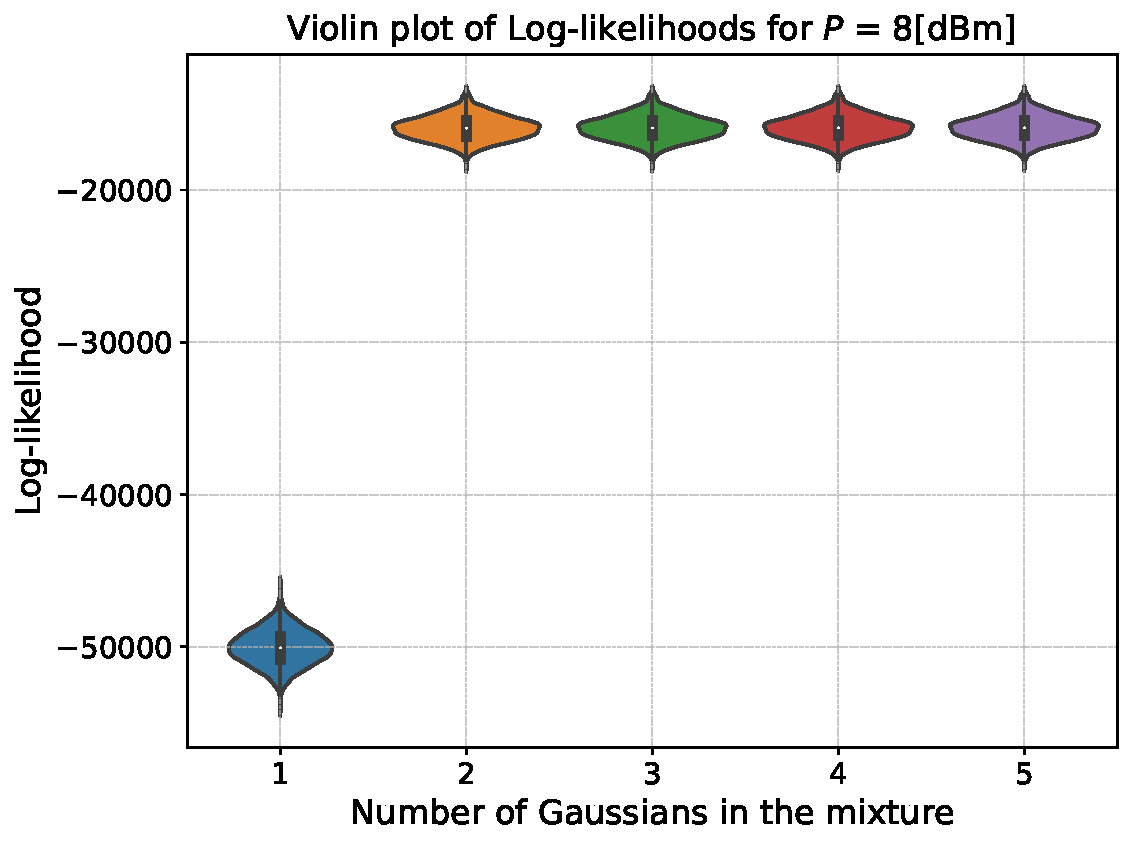
\includegraphics[width=1\linewidth]{images/gauss/bigf_loglik_pdbm_8.pdf} (f) \\
    }
    \end{minipage}

    \caption{Violin plot of log-likelihood for triplet distribution for different number of components in \gls{gmm}. \textbf{(a)} $P_{ave} = -2$ $\mathrm{[dBm]}$, \textbf{(b)} $P_{ave} = 0$ $\mathrm{[dBm]}$, \textbf{(c)} $P_{ave} = 2$ $\mathrm{[dBm]}$, \textbf{(d)} $P_{ave} = 4$ $\mathrm{[dBm]}$, \textbf{(e)} $P_{ave} = 6$ $\mathrm{[dBm]}$, \textbf{(f)} $P_{ave} = 8$ $\mathrm{[dBm]}$ }
    \label{fig:violin_different_power}
\end{figure}